\chapter{Кристаллы, дефекты и границы}

\section{Гексагональная решётка циркония}

Ниже 863\degC{} цирконий имеет \textbf{гексагональную плотноупакованную} (ГПУ) решётку --- $\alpha$-Zr.
Её ячейка --- шестигранная призма (рис.~\ref{fig:f4_hcp}а) с параметрами $a \approx 0.323$~нм в основании и
$c\approx 0.515$~нм по высоте; отношение $c/a\approx1.593$ немного меньше идеального $\sqrt{8/3}=1.633$.

Плоскости и направления в ГПУ удобно обозначать четырьмя индексами Миллера--Браве $(hkil)$ с $i = -(h+k)$:
три оси $a_1, a_2, a_3$ в базисной плоскости под 120\textdegree{} и ось $c$. Лишний индекс нужен, чтобы
одинаковые по симметрии плоскости и выглядели одинаково. Важнейшие плоскости:
\begin{itemize}
\item \textbf{базисная} $(0001)$ --- перпендикулярна оси $c$;
\item \textbf{призматические} $\{10\bar10\}$ --- боковые грани призмы, параллельны $c$;
\item \textbf{пирамидальные} $\{10\bar1l\}$ --- наклонные. Плоскость $\{10\bar17\}$, около которой лежат
  гидриды, всего на 15\textdegree{} отклонена от базисной.
\end{itemize}

\fig{f4_hcp}{а) Ячейка ГПУ $\alpha$-Zr: базисная плоскость $(0001)$ (синяя), призматическая $\{10\bar10\}$
(красная), оси $a_1$--$a_3$ и $c$. б) Пластинка $\delta$-гидрида на плоскости, близкой к базисной: в плоскости
пластинки гидрид шире матрицы на $\approx4.6\,\%$, поперёк неё --- на $\approx7.2\,\%$.}

\begin{idea}
ГПУ решётка сильно \emph{анизотропна}: свойства вдоль $c$ и поперёк различаются. Тепловое расширение вдоль
$c$ заметно больше, чем в базисной плоскости. Скольжение дислокаций легко идёт по призматическим плоскостям и
трудно --- с компонентой вдоль $c$. Поэтому то, как ориентированы оси $c$ зёрен (текстура, глава~7), определяет и
прочность трубы, и то, как в ней лягут гидриды.
\end{idea}

\section{Гидриды циркония}

У циркония несколько гидридов:
\begin{itemize}
\item $\delta$-ZrH$_{1.5\ldots1.7}$ --- основной в оболочках. Решётка гранецентрированная кубическая (типа
  флюорита), $a\approx0.478$~нм. Водород занимает тетраэдрические пустоты.
\item $\gamma$-ZrH --- гранецентрированная тетрагональная; метастабильная, появляется при быстром охлаждении.
\item $\varepsilon$-ZrH$_2$ --- при очень высоком водороде.
\end{itemize}
$\delta$-гидрид выпадает с ориентационным соотношением $(0001)_\alpha\parallel\{111\}_\delta$,
$\langle11\bar20\rangle_\alpha\parallel\langle110\rangle_\delta$: плотноупакованные плоскости обеих решёток
параллельны. При таком сопряжении гидрид шире матрицы на $\eps_a\approx4.6\,\%$ в базисной плоскости и на
$\eps_c\approx7.2\,\%$ вдоль оси $c$; объём больше на $\approx17\,\%$ (Carpenter, 1973).

\begin{zrbox}
Гидрид, видимый на шлифе как одна линия длиной в десятки--сотни микрометров, на самом деле --- пачка тонких
\emph{микропластинок} толщиной 0.1--1~мкм и длиной в единицы микрометров. Они лежат около $\{10\bar17\}$ внутри зёрен
и цепляются друг за друга, переходя из зерна в зерно. Модель работает именно с микропластинками, а «макрогидрид»
--- результат их коллективного расположения.
\end{zrbox}

\section{Точечные дефекты}

Даже идеальный кристалл при $T>0$ содержит \textbf{вакансии} --- пустые узлы. Их равновесная доля
\begin{equation}
c_v = e^{S_f/k_B}\,e^{-H_f/k_BT},
\end{equation}
$H_f\sim1$--2~эВ, у точки плавления $c_v\sim10^{-4}$. Образование вакансии стоит энергии, но приносит
энтропию --- та же борьба $H$ и $TS$, что и в главе~1. Атомы \textbf{внедрения} (водород, кислород, углерод)
сидят в пустотах между узлами. Именно поэтому водород не нуждается в вакансиях, чтобы двигаться.

\section{Дислокации}

Пластическая деформация металла идёт не сдвигом целых атомных плоскостей разом (на это нужны напряжения порядка
$\mu/10$, в сотни раз больше реальных), а движением \textbf{дислокаций} --- линейных дефектов, вдоль которых
одна часть кристалла уже сдвинута относительно другой.

Проще всего представить \textbf{краевую дислокацию}: в кристалл сверху вставлена лишняя полуплоскость атомов,
обрывающаяся на плоскости скольжения (рис.~\ref{fig:f4_dislocation}а). Сдвиг, который несёт дислокация, задаёт
\textbf{вектор Бюргерса} $\mathbf b$; в цирконии для лёгкого скольжения $\mathbf b = \tfrac13\langle11\bar20\rangle$,
$|\mathbf b| = a$. Когда дислокация проходит через кристалл, верхняя половина сдвигается на $\mathbf b$.

\fig{f4_dislocation}{а) Краевая дислокация: над плоскостью скольжения вставлена лишняя полуплоскость (красные
атомы), соседние столбцы раздвинуты. б) Напряжение $\sigma_{xx}$ вокруг неё (изотропная теория упругости): над
плоскостью скольжения --- сжатие, под ней --- растяжение; убывает как $1/r$.}

Вокруг дислокации решётка искажена, и её поле напряжений спадает как $1/r$:
\begin{equation}
\sigma_{xx} = -\frac{\mu b}{2\pi(1-\nu)}\,\frac{y\,(3x^2+y^2)}{(x^2+y^2)^2}.
\end{equation}
Энергия дислокации на единицу длины $\approx \mu b^2/2$ --- несколько эВ на каждое межатомное расстояние. Поэтому
дислокации никогда не находятся в равновесии: они появляются при деформации и остаются, пока их не уберёт отжиг.

\begin{zrbox}
Дислокации важны для гидридов трижды:
\begin{itemize}
\item в растянутой области под краевой дислокацией водороду «просторнее» (глава~3), и туда он стекается ---
  дислокации служат местами зарождения гидридов;
\item гидрид при выпадении сам рождает дислокации вокруг себя: его несоответствие слишком велико, чтобы матрица
  выдержала его упруго (глава~7);
\item эти дислокации остаются после растворения гидрида и «помнят» его место --- при следующем охлаждении гидрид
  выпадает там же. Это \textbf{эффект памяти}.
\end{itemize}
\end{zrbox}

\section{Межфазные границы}

Граница между матрицей и выделением бывает трёх типов (рис.~\ref{fig:f4_interfaces}).
\begin{itemize}
\item \textbf{Когерентная}: атомные плоскости непрерывно переходят через границу; несоответствие решёток
  снимается упругим искажением. Энергия границы мала (0.05--0.2~Дж/м$^2$), но упругая энергия велика и растёт с
  объёмом выделения.
\item \textbf{Полукогерентная}: несоответствие частично снято \textbf{дислокациями несоответствия}, по одной на
  каждые $b/\delta$ плоскостей, где $\delta = (a_\beta - a_\alpha)/a_\alpha$. Энергия границы выше (0.2--0.5).
\item \textbf{Некогерентная}: решётки никак не сопряжены. Энергия границы велика (0.5--1), зато упругое поле
  почти снимается.
\end{itemize}

\fig{f4_interfaces}{Типы межфазных границ: а) когерентная --- решётка выделения подстроена под матрицу;
б) полукогерентная --- периодические дислокации несоответствия ($\perp$); в) некогерентная.}

\begin{idea}
Выделение выбирает компромисс между энергией границы (растёт как площадь, $\propto r^2$) и упругой энергией
(растёт как объём, $\propto r^3$). Маленький зародыш почти всегда когерентен: граница дешёвая, а упругая энергия
при малом объёме ещё невелика. Большой гидрид теряет когерентность, рождая дислокации.
\end{idea}

\section{Границы зёрен}

Металл трубы --- поликристалл из зёрен в несколько микрометров с разной ориентацией решётки. На стыке двух зёрен
--- \textbf{граница зерна}. При малой разориентации $\theta$ это просто стенка дислокаций, и её энергия растёт по
формуле Рида--Шокли $\gamma = \gamma_m(\theta/\theta_m)\bigl(1-\ln(\theta/\theta_m)\bigr)$. При $\theta\gtrsim15^\circ$
дислокации сливаются, и энергия выходит на плато $\gamma_m\approx0.5$--1~Дж/м$^2$ с провалами у особых
разориентаций (рис.~\ref{fig:f4_gb}).

\begin{figure}[htbp]\centering
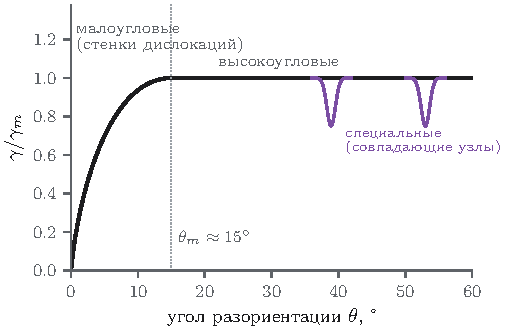
\includegraphics[width=0.6\linewidth]{f4_gb}
\caption{Энергия границы зерна от угла разориентации: рост по Риду--Шокли для малоугловых границ, плато для
высокоугловых, провалы у специальных разориентаций (совпадающих узлов) --- условно.}
\label{fig:f4_gb}
\end{figure}

\begin{zrbox}
Границы зёрен --- готовые места для зарождения: часть энергии границы «уходит в дело», когда на ней вырастает
выделение (глава~6). Гидриды часто выпадают на границах, и межзёренные гидриды могут быть ориентированы иначе, чем
внутризёренные, привязанные к базисной плоскости своего зерна (Qin и др., 2011; Wang и др., 2019). Это ещё один
путь к радиальным гидридам, когда внутри зёрен им мешает текстура.
\end{zrbox}

\begin{exercise}
Найдите угол между нормалью к плоскости $(10\bar17)$ и осью $c$ в ГПУ с $c/a = 1.593$. (Подсказка: для плоскости
$(hkil)$ угол $\varphi$ с базисом даёт $\operatorname{tg}\varphi = \tfrac{2}{\sqrt3}\,\tfrac{c}{a}\,\sqrt{h^2+hk+k^2}/l$.)
\end{exercise}

\begin{exercise}
Объёмное несоответствие гидрида 17\,\%. Сколько это в линейном несоответствии, если считать его изотропным? Через
сколько межплоскостных расстояний пришлось бы ставить дислокацию несоответствия, чтобы снять его полностью?
\end{exercise}

\begin{exercise}
Оцените энергию дислокации на единицу длины при $\mu = 33$~ГПа, $b = 0.323$~нм. Сколько это в эВ на межатомное
расстояние?
\end{exercise}
